\section{Accepttest}
\label{volumenkontrol-accepttest}
Det kan konkluderes at VCO'en fungerer som simuleret, og denne må derfor ses som en succes. Tælleren fungerer derimod ikke tilfredsstillende. Den kan i enkelte tilfælde tælle op til 51. Årsagen til fejlen er ikke lokaliseret. Desuden tæller den i nogle tilfælde op, selvom den burde tælle ned. Dette er dog ikke tilfældet, hvis knappen holdes inde. Årsagen til denne fejl er heller ikke lokaliseret. Tælleren ses derfor som ikke at leve op til kravet. Displayet samt displaydriverne fungerer og viser de rigtige tal ud fra det input de får.

Dæmpningen af signalet fungerer som forventet, se Appendiks \ref{maalevolumenkontrol}. THD-målingerne i volumenkontrol viser at den, ved højeste volumen, er under 0,01\% på sit højeste, som set på figur \ref{fig:accvold:thd0}. Dette accepteres, da dette er lavt i forhold til de 1\%, som er maksimum for hele systemet. 
\begin{figure}[h]
\centering
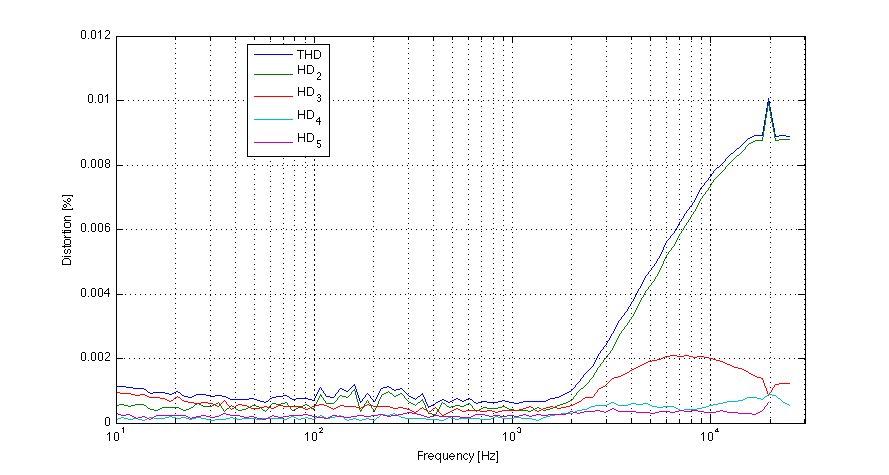
\includegraphics[width=\textwidth]{maalerapporter/volumenkontrol/2Vniveau0-thd.png}
\caption{THD for volumenkontrollen ved fuldt signal}
\label{fig:accvold:thd0}
\end{figure}

Der findes ved måling, at volumenkontrollen, uden dæmpning, forstærker 0,0027 dB ved 1 kHz. Dette sammenlignes med 0,0021 dB 20 Hz og -0,0015 dB ved 20 kHz. Dette giver en maksimalt afvigelse fra referencefrekvens 1 kHz på 0,0042 dB. Dæmpningsdelen af volumenkontrollen er derfor accepteret.
\begin{figure}[h]
\centering
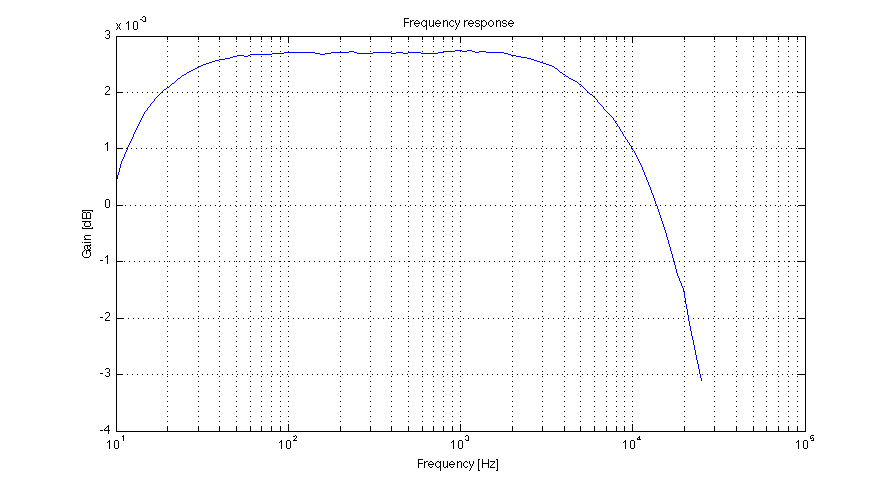
\includegraphics[width=\textwidth]{maalerapporter/volumenkontrol/2Vniveau0-frek.png}
\caption{Frekvensgang for volumenkontrollen ved fuldt signal}
\label{fig:accvold:frek0}
\end{figure}


\begin{table}[h]
\centering
\begin{tabular}{l|r|r}
\hline\hline
Område & Krav & Status \\
\hline\hline
Frekvensgang & $\pm$ 0,375 dB ved 20 Hz - 20 kHz, ref. 1 kHz & \checkmark \\
& $\pm$ 0,75 dB fra 20 Hz til 63 Hz & \checkmark \\
& $\pm$ 0,75 dB fra 12,5 kHz til 20 kHz & \checkmark \\[4pt]
Dæmpningsområde i & 0 - 50 dB ved 1 kHz & \checkmark \\
volumenkontrol && \\[4pt]
Styring af volumen- & Digital & \checkmark \\
kontrol && \\[4pt]
Antal niveauer i & 51 & $\mathcal{X}$ \\
volumenkontrollen && \\[4pt]
Dæmpning per & 1 dB & \checkmark \\
niveau && \\[4pt]
Input fra brugeren & To trykknapper & \checkmark \\[4pt]
Output til brugeren & To 7-segmenter & \checkmark \\
\hline\hline
\end{tabular}
\caption{Oversigt over status af krav til volumenkontrollen}
\label{tab:krav_volumenkontrol}
\end{table}
